%%
%% $Id$
%%
%% Copyright (c) 2007-2008 Christian Fehler
%% Copyright (c) 2007-2008 Benjamin Mies
%%


\chapter{Minimierung}\label{Minimize}

Sobald der Benutzer einen Automaten erstellt hat, kann er mit diesem schon alle
Funktionen, welche dieses Lernwerkzeug bietet, nutzen. Allerdings besteht die
Möglichkeit, dass ein Automat existiert, der die gleiche Sprache erkennt, die ein
erstellter Automat erkennt, jedoch mit weniger Zuständen auskommt. Bei
komplexeren Beispielen bemerkt man schnell, dass die Übersichtlichkeit mit
wachsender Anzahl der Zustände immer weiter abnimmt. Daher ist es wünschenswert,
immer mit dem minimalen Automaten für eine bestimmte Sprache zu arbeiten. Im
Folgenden wollen wir uns jetzt den Algorithmus ansehen, welcher verwendet wird,
um aus einem Automaten einen neuen Automaten mit einer minimalen Anzahl von
Zuständen zu erzeugen. Dieser Algorithmus ist aus \cite{Compilers}
entnommen. In Abbildung \ref{FigureMinimization} sieht man wie die
Minimierung im GTI Tool graphisch dargestellt wird.\vspace{10pt}

Wie bereits erwähnt, erwartet der Algorithmus als Eingabe einen Automaten, und
erzeugt als Ausgabe einen neuen Automaten welcher die gleiche Sprache
akzeptiert, jedoch mit einer minimalen Anzahl von Zuständen
auskommt.\vspace{10pt}

Der erster Minimierungsschritt besteht darin, die unerreichbaren Zustände zu
entfernen, da diese keine Auswirkung auf die erkannte Sprache haben können. Der
dazu verwendete Algorithmus zur Berechnung der erreichbaren Zustände kann im
Abschnitt \ref{ReachableStates} nachgeschlagen werden.\vspace{10pt}

Im Weiteren versuchen wir, äquivalente Zustände in Gruppen, auch
Äquivalenz\-klassen genannt, zusammenzufassen, um diese später zu einem Zustand
zu verschmelzen. Um herauszufinden, ob zwei Zustände in der gleichen
Äquivalenz\-klasse liegen, überprüft man für jedes Symbol des Alphabets
einzeln, ob alle Zustände der Gruppe mit diesem Symbol in Zustände der selben
Gruppe übergehen.\vspace{10pt}

Initial wird unsere Menge von Zuständen in zwei Gruppen unterteilt. Alle
akzeptierenden Zustände bilden die erste, alle nicht akzeptierenden Zustände die
zweite Gruppe.\vspace{10pt}

Der Algorithmus nimmt sich jetzt das Alphabet des Eingabeautomaten zur Hilfe, um
zu prüfen, ob alle Zustände einer Gruppe wirklich in einer Äquivalenzklasse
liegen, oder ob wir die Gruppe aufspalten müssen. Dazu sei gesagt, dass zwei
Zustände in der selben Äquivalenzklasse liegen, wenn sie mit jeweils allen
Symbolen des Eingabealphabets in einen Zustand der selben Gruppe
übergehen.\vspace{10pt}

\begin{figure}[h]
\begin{center}
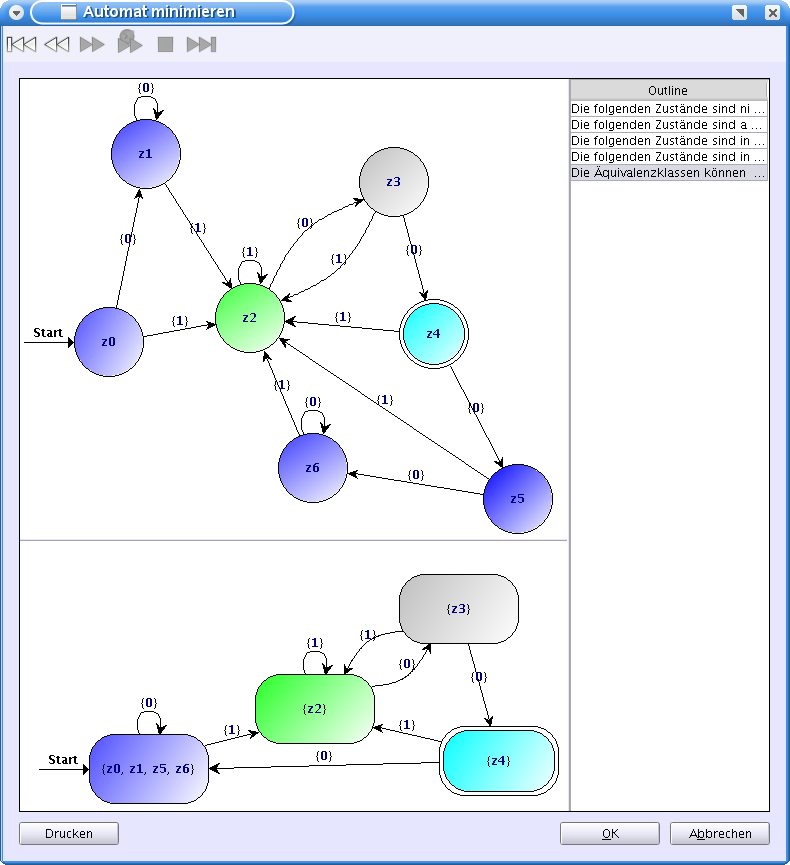
\includegraphics[width=12cm]{../images/minimize.png}
\caption{Automat - Minimierung}
\label{FigureMinimization}
\end{center}
\end{figure}
\vspace{10pt}

Schauen wir uns jetzt mal die Arbeitsweise des Algorithmus im Detail an. Als
erstes wird die aktuelle Gruppeneinteilung gespeichert, also wie viele
Gruppen existieren, und welcher Zustand in welcher Gruppe liegt. Dann wird
die erste Gruppen betrachtet. Wenn diese nur einen Zustand enthält, kann sie
nicht weiter verfeinert werden, und muss daher auch nicht mehr betrachtet werden.
\vspace{10pt}

Enthält die Gruppe mehr als einen Zustand, wird das aktuelle Alphabet des
Automaten betrachtet. Der Algorithmus überprüft jetzt, ob alle Zustände dieser
Gruppe in der gleichen Äquivalenzklasse liegen. Wenn das der Fall ist, kann auch
diese Gruppe nicht weiter unterteilt werden. Falls aber doch Zustände
existieren, welche in einer anderen Äquivalenz\-klasse liegen, werden diese
Zustände aus der aktuellen Gruppe entfernt und bilden eine neue Gruppe. \vspace{10pt}

Nachdem diese Prozedur für die aktuelle Gruppe abgeschlossen ist, wird sie für
alle Gruppen, die noch nicht betrachtet wurden, wiederholt. Nach Betrachtung aller
Gruppen wird die aktuelle Gruppeneinteilung mit der verglichen, die zu Beginn
gespeichert wurde. Wenn diese übereinstimmt, ist unser Algorithmus am Ende, und
die Gruppen können nicht weiter verfeinert werden. Stimmt die Gruppeneinteilung
nicht überein, muss jede Gruppe erneut einzeln betrachten, um zu versuchen,
diese in kleinere Gruppen zu zerlegen.\vspace{10pt}

Nach Beendigung des Algorithmus repräsentiert jede Gruppe einen Zustand
im minimalen Automaten. Jetzt muss noch pro Symbol des Alphabets der
Übergang in den entsprechenden neuen Zustand angelegt werden. Mit diesem
letzten Schritt ist die Konstruktion des minimalen Automaten
abgeschlossen.\vspace{10pt}

In unserem Lernwerkzeug wird dem Benutzer wie üblich in der Outline angezeigt,
was in den bisherigen Schritten des Algorithmus passiert ist.\vspace{10pt}
